% Created by Christoph Jansen
% License: CC BY 4.0 http://creativecommons.org/licenses/by/4.0/
% Source: https://github.com/Gnork/htw-latex-template
% THIS TEMPLATE IS NOT OFFICIAL
% Offical .doc template: http://www.htw-berlin.de/hochschulstruktur/zentrale-referate/presse-und-oeffentlichkeitsarbeit/abschlussarbeiten-vorlagen/

\documentclass[12pt, a4paper]{book}
\usepackage[twoside=false,margin=2.5cm,bindingoffset=2cm]{geometry}

\usepackage[utf8]{inputenc}
%\usepackage{bibgerm}
\usepackage{natbib}
\usepackage{ngerman}
\usepackage{graphicx}
\usepackage{wallpaper}
\usepackage{textpos}
\usepackage{fancyvrb}
\usepackage{listings}
\usepackage{hyperref}
\usepackage{changepage}
\usepackage{xcolor}

\hypersetup{
  colorlinks   = true,    % Colours links instead of ugly boxes
  urlcolor     = blue,    % Colour for external hyperlinks
  linkcolor    = black,    % Colour of internal links
  citecolor    = black      % Colour of citations
}
\lstset{
    basicstyle=\ttfamily,    % Schriftart
    breaklines=true,         % Automatischer Zeilenumbruch
    breakindent=0pt,         % Keine Einrückung beim Zeilenumbruch
    breakatwhitespace=false, % Zeilenumbrüche können an jedem Zeichen erfolgen
    frame=none,              % Kein Rahmen um den Code
    xleftmargin=0pt,         % Keine Einrückung auf der linken Seite
    xrightmargin=0pt,        % Keine Einrückung auf der rechten Seite
    tabsize=4,               % Tabulatorgröße
    captionpos=b             % Position der Beschriftung (unten)
}

% set wallpaper position for title page
\addtolength{\wpXoffset}{0.0cm}
\addtolength{\wpYoffset}{7.0cm}

% define htw color for title page
\definecolor{htwgreen}{RGB}{118,185,0}
% % Inhaltsverezichnis Stil - Abstand zw. Punkten und dem Überschrift und Verzeichnis
\setlength{\cftaftertoctitleskip}{30pt}
\renewcommand{\cftdotsep}{2.5}
\renewcommand{\cftsecleader}{\cftdotfill{\cftdotsep}}
% % Seitenstil für die Titelseite definieren (leere Kopf- und Fußzeile)
% \fancypagestyle{titlestyle}{
%   \fancyhf{} % clear all header and footer fields
%   \renewcommand{\headrulewidth}{0pt} % remove the header rule
%   \renewcommand{\footrulewidth}{0pt} % remove the footer rule
% }

% % Seitenstil für den Hauptteil definieren
% \pagestyle{fancy}
% \fancyhf{} % clear all header and footer fields
% \fancyhead[C]{\leftmark} % zentrierte Kopfzeile mit dem Namen des aktuellen Kapitels
% \renewcommand{\headrulewidth}{0.4pt} % Linie unter der Kopfzeile
% \renewcommand{\footrulewidth}{0pt} % keine Linie unter der Fußzeile

% Anpassung der Kapitelmarkierung, um die Section anzuzeigen statt Chapter
\renewcommand{\sectionmark}[1]{\markboth{#1}{}}

\begin{document}

% Titelseite mit speziellem Seitenstil
% \thispagestyle{titlestyle}
\begin{titlepage}
%\ThisCenterWallPaper{1.0}{images/titel.jpg}

\title{
\date{}
\vspace*{-50mm} 
{
\includegraphics{images/htw_logo.jpg}}\\

\vspace{1.2cm}
\hrulefill 
\vspace{0.5cm}
\textcolor{htwgreen}{
{\textbf{\Large \\ Konzeption und Entwicklung eines Showcases zur Integration eines Geoinformationssystems in das Formularmanagementsystem am Beispiel eines Schulanmeldeformulars für NRW}}}\\
\hrulefill 
\vspace{0.5cm}

{\normalsize Bachelorarbeit}\\
{\normalsize zur Erlangung des akademischen Grades}\\
{\large Bachelor of Science (B.Sc.) }\\
\vspace{1.2cm}

{\normalsize an der}\\
{\normalsize Hochschule für Technik und Wirtschaft Berlin}\\
{\normalsize Fachbereich 4 Informatik, Kommunikation und Wirtschaft}\\
{\normalsize Studiengang Informatik und Wirtschaft}\\
\vspace{1.2cm}
\normalsize Erstgutachter: Prof. Dr.-Ing. Jörn Freiheit \\
\normalsize Zweitgutachter:  Dr. Christian Kudla \\
\vspace{1.2cm}

\normalsize Eingereicht von:\\
\large Radmila Heizenreder\\
\vspace{0.2cm}
\normalsize Berlin, \today \\
\vspace{-100mm}
}

\maketitle
\end{titlepage}
\frontmatter
% \section*{Leitfaden}
Abstract:
•	Das Abstract fasst die wesentlichen Inhalte Ihrer Bachelorarbeit zusammen, ohne diese zu werten oder zu interpretieren.
•	Bietet einen groben Überblick über Ihre Fragestellung, Ihr Vorgehen und Ihre zentralen Ergebnisse
•	Wird am Ende geschrieben.

Das Abstract enthält:
1.	-Hintergrundinformationen (z. B. Ausgangslage, Fragestellung und Zielsetzung der Arbeit, Relevanz/
2.	Forschungskontext, entspricht der Einleitung der Arbeit)
3.	-Forschungsmethoden/ Vorgehen, evtl. kurze Benennung der Thesen, bei empirischen Studien auch Angaben zu den Daten wie etwa die Charakteristika der Stichprobe.
4.	-Ergebnisse
5.	-Schlussfolgerungen, Implikationen oder Anwendungsmöglichkeiten (entspricht dem Diskussionsteil der Arbeit) 
6.	-Inhalt knapp, vollständig und präzise wiedergeben
7.	-Fokus auf das Wesentliche
8.	-Objektiv, einfach, verständlich formulieren
9.	-Keine Nennung des Titels, keine Zitate
10.	-Umfang in der Regel 150 bis 250 Wörter ->ggf. Betreuer*in fragen

Insgesamt ca. 5 Sätze zu folgenden Punkten (keine bestimmte Reihenfolge): 
1.	Was war das Ziel und die Fragestellung der Arbeit? 
2.	Welche Methode(n) wurden verwendet? 
3.	Was waren die wichtigsten Konzepte und Quellen, auf denen die Arbeit basiert? 
4.	Was waren die wichtigsten Ergebnisse der Arbeit, und was folgt daraus? 
5.	Ggf. kurze Verortung des Themas in einem allgemeinen Kontext



Einleitung
•	Um welchen Themenbereich handelt es sich?
•	Warum ist es relevant, sich mit diesem Themenbereich zu befassen?
•	Was hat die Forschung zu diesem Themenbereich an Erkenntnissen gewonnen?
•	Wie wurden die vorhandenen Erkenntnisse gewonnen?
•	Welche Fragen sind bislang offen geblieben?
•	Welche dieser offenen Fragen ist Gegenstand der vorliegenden Untersuchung?
•	Wie werden die neuen Erkenntnisse gewonnen?
•	Welche neuen Erkenntnisse sollen gewonnen werden?
•	Wie sind die zu erwartenden neuen Erkenntnisse im Zusammenhang mit den bereits vorhandenen Erkenntnissen einzuschaetzen?
•	Welche Rahmenbedingungen muessen beachtet werden?
•	Wie ist die Arbeit angelegt?


	Verbindung zum Allgemeinen herstellen - In welchem übergeordneten Thema und vor welcher fachspezifischen Herausforderung ist die Arbeit verortet? Hier sollten Sie ein wissenschaftliches, aber u.U. fachfremdes Lesepublikum abholen und in Ihren Bereich des Themas einführen.
	Forschungsstand zusammenfassen und Forschungslücke identifizieren - Was wurde zu diesem Themenbereich schon untersucht, und was noch nicht? Hier also eine kurze Zusammenfassung des Kapitels Forschungsstand und theoretische Grundlagen. 
	Ziel und Fragestellung benennen - Welchen Teilaspekt des Themas möchten Sie innerhalb dieser Arbeit untersuchen und warum? Was unterscheidet Ihre Arbeit von anderen Arbeiten zu ähnlichen Themen? 
	Ggf. Hypothese formulieren - Formulieren Sie noch vor der Durchführung Deiner Untersuchung eine begründete Vermutung, welche Antwort auf Ihre Fragestellung anhand des Forschungsstandes am wahrscheinlichsten ist. (Wenn Sie eine explorative Arbeit schreiben, gehen Sie anders vor: dann ist es Ziel der Arbeit, eine Hypothese anhand der Untersuchungsergebnisse zu formulieren.) 
	Überblick zum Aufbau geben - Kurze Info über Kapitelinhalte: Was sollen sie zur Beantwortung der Forschungsfrage beitragen?
	Abkürzungen erklären - Wenn Sie Abkürzungen verwenden, schreiben Sie sie das erste Mal ganz aus. Gemeint sind damit nicht reguläre Abkürzungen wie ‚z.B.‘ für ‚zum Beispiel’, sondern Akronyme wie ‚AMA‘ für ‚American Marketing Association’. Bei vielen Abkürzungen sollten Sie ein separates Abkürzungsverzeichnis anlegen.


\begin{abstract}
Jedes Kapitel sollte eine Überleitung und wenn möglich auch ein Zwischenfazit oder eine kurze Zusammenfassung haben: 
\begin{itemize}
    \item Welchen logischen Bezug hat das aktuelle Kapitel zum vorherigen oder nächsten Kapitel?
    \item Was waren die wichtigsten Erkenntnisse und die Hauptaussage in diesem Kapitel?
    \item Was trägt dieses Kapitel zur Beantwortung der Forschungsfrage bei?
\end{itemize}
\end{abstract}


Code-Snippsel:
Dies ist ein Beispiel für \Verb|code in einer Zeile|, der auch Sonderzeichen wie

zitieren \citep{Bleek.2005} ==> (Bleek 2005)==================
zitieren \citet{Bleek.2005} ==> Bleek (2005)==================
zitieren \citep[S.~373]{Lange.2020} ==================


(Abs.~\ref{sec:Form.io})
\chapter{Eigenständigkeitserklärung}
\noindent Ich erkläre hiermit, dass
\begin{itemize}
    \item ich die vorliegende wissenschaftliche Arbeit selbständig und ohne unerlaubte Hilfe angefertigt habe,
    \item ich andere als die angegebenen Quellen und Hilfsmittel nicht benutzt habe,
    \item ich die den benutzten Quellen wörtlich oder inhaltlich entnommenen Stellen als solche kenntlich gemacht habe,
    \item die Arbeit in gleicher oder ähnlicher Form noch keiner anderen Prüfbehörde vorgelegen hat.
\end{itemize}
\vspace{2cm}
% \noindent 
\begin{tabular}{@{}p{\dimexpr 0.5\textwidth-\tabcolsep}p{\dimexpr 0.5\textwidth-\tabcolsep}@{}}
    Berlin, \today & \hfill \rule{6cm}{0.4pt} \\
    & \hfill Radmila Heizenreder \\
\end{tabular}


\chapter{Kurzeschreibung}
\tableofcontents
\listoffigures
\mainmatter
\chapter{Einleitung}
\label{cha:einleitung}

% - item Welche Themen grenzen an meine Fragestellung?
% - Welche Begriffe und Konzepte sind relevant für mein Thema?
% - Welche Theorien oder liegen meiner Untersuchung zu Grunde?
% - Welche relevanten Arbeiten gibt es zu diesen Themen?
% - Welche Ergebnisse liefern diese Arbeiten? ? Welche Gemeinsamkeiten und Unterschiede zeigen sich darin?
% - Was kann ich aus diesen Ergebnissen schließen? Welche Frage will ich also konkret beantworten? Bzw. Welche Aufgabe will ich umsetzen?



% digitalisierung in deutschland
% OZG
% Telekom macht onlinedienste zugänglich
% die antragstellung in dem digitalisierungsprozess
% um online antrag zu bauen, gibt es einege Lösungen - fms
% um in der Antragstrecke formulare zu überpfrüfen/validieren, muss das Formular mehr können als bis jetzt
% anhand eines Showcases wird geforscht, ob geodaten und deren bearbeitung ins formular integrieren lässt

\section{Motivation}
%Verwaltungsdigitalisierung in Deutschland
%OZG und Telekom
%Ziel - Formulare eine weitere Funktionalität zu schaffen\\
In unserer Zeit, die nicht nur durch den digitalen Wandel, sondern auch durch die Herausforderungen der Covid-19-Pandemie geprägt ist, hat sich die Bedeutung digitaler Technologien dramatisch verstärkt. Mit der stetigen Weiterentwicklung mobiler Endgeräten hat sich unser Alltag tiefgreifend geändert. Wir nutzen diese Technologien nicht nur für Kommunikation und Unterhaltung, sondern auch für Bildung und Geschäftliches. Insbesondere während der Pandemie hat sich gezeigt, wie unverzichtbar digitale Lösungen für die Aufrechterhaltung des sozialen und wirtschaftlichen Lebens sind.\\


In diesem Kontext streben auch Behörde danach, ihre Dienste online anzubieten, um mit der globalen Entwicklungen und den durch die Pandemie verstärkten Anforderungen an digitale Zugänglichkeit Schritt zu halten. In Deutschland bildet das 2017 einfgeführte Onlinezugangsgesetz (OZG) die rechtliche Grundlage für diese Transformation. Das OZG, ein Gesetz zur Verbesserung des Onlinezugangs zu Verwaltungsleistungen, verpflichtet seitdem Bund, Länder und Kommunalbehörden dazu, ihre Dienstleistungen auch elektronisch über Verwaltungsportale bereitszustellen \citep{bundesministerium_des_innern_und_fur_heimat_onlinezugangsgesetz_2017}. Ziel des OZG ist es, den Bürgern und Unternehmen einen einfacheren und effizienteren Zugang zu Verwaltungsleistugen zu bieten. Es ermöglicht den Bürgern, Anträge und Formulare sowie andere Verwaltungsprozesse online zu erledigen.\\

Eines der wichtigesten Schlüsselelemente in dieser digitalen Transformation ist ein leistungsfähiges Formularmanagementsystem (FMS). Hier spielt das von der Telekom MMS GmbH weiterentwickelte Open Source form.io \citep{formio} eine zentrale Rolle für die Entwicklung des Verwaltungsportals in NRW. Es unterstützt die Digitalisierung von Papierformularen und trägt zu einer effizienten, modernen IT-Infrastruktur bei.\\

``Digitalisierung bedeutet in der Folge, analoge Informationen in digitale Daten umzuwandeln'' \cite[S.~90]{markus_auf_2022}
Die Digitalisierung der Papierformulare, welche durch das FMS form.io ermöglicht wird, hat das Potenzial, nicht nur die Effizienz zu steigern, sondern auch die Benutzererfahrung zu verbessern. Ein innovativer Ansatz in diesem Bereich ist die Integration dynamische Elemente in digitale Formulare. Beispielsweise können abhängig von den Benutzereingaben unterschiedliche Eingabebereiche ein- oder ausgeblendet werden. Weiterhin bietet das FMS die Möglichkeit, Daten aus Datenbanken abzurufen und die Eingabefelder vorzubefüllen. Die Antragsstellende können somit relevante Daten einsehen, bearbeiten und direkt im Formular übernehmen.\\



% wie digitalisieren sich behörde und ihre dienste? 



 
\section{Ausgangssituation und Aufgabenstellung}
\label{sec:forschung}
% ``Die Digitalisierung der Verwaltung basiert auf den Visionen, die bereits vor vielen Jahren u.a. in Bezug auf medienbruchfreie, ubiquitäre, digitale Antragsmöglichkeiten für Bürger:innen skizziert wurde. Die Digitalisierung folgt den Digitalisierungsstrategien der Beteiligten u.a. auf den föderalen Ebenen.'' \cite[S.~21]{lohmann_architekturrahmen_2021}\\

Seit einigen Jahren wird das Verwaltungsdenken von dem Schlagwort Kundenorientierung beflügelt. Gesucht sind Herangehensweisen und Verfahren, die bei der Entwicklung von E-Government-Dienstleistungen systematisch und nachhaltig die Anliegen der potenziellen Nutzer wie Bürger:innen oder Unternehmen im jeweiligen Zuständigkeitsbereich einbeziehen und zu gesicherter Akzeptanz der Online-Angebote führen \citep{bleek_steuerungsmodell_2005}.\\

Die Deutsche Telekom MMS GmbH, im Folgenden nur „Telekom MMS“ genannt, entwickelt seit einigen Jahren Verwaltungsportale für NRW. Einige Formulare dort sind mit FMS Form.io modelliert worden und es wurden einige Funktionalitäten realisiert, die das Ausfüllen des Antragskomfortabler für die BürgerInnen machen. Im Rahmen dieser Bachelorarbeit werde ich für das Unternehmen ein Showcase entwerfen und den Funktionsumfang des FMS erweitern, indem eine neue Funktionalität ins Formular integriert wird.\\

Heutzutage ist unsere Welt ohne Maps, Geodaten und Navigation nicht mehr vorstellbar. Die Nutzung von Geoinformationen spielt mittlerweile in allen Bereichen – sowohl in der Wissenschaft, der öffentlichen Verwaltung, der Wirtschaft, Politik als auch im privaten Leben – eine wichtige Rolle. Daher wird in der Arbeit die Forschungsfrage gestellt und untersucht, ob und welches geografische Informationssystem in das FMS form.io als neue Funktionalität integriert werden kann und inwieweit dieses die Verwaltungsprozesse unterstützt.\\

Ich schreibe somit über die Konzeption und Implementierung eines Showcases zur Integration eines GIS in das FMS Form.io am Beispielformular Schulanmeldung in der Stadt Münster. Ich möchte verstehen, welche technischen und praktischen Herausforderungen bei der Einbettung geografischer Informationssysteme in Online-Formulare bestehen und wie diese effizient gelöst werden können. Dabei möchte ich herausfinden, welche Vorteile die GIS-Integration für die Datenvisualisierung und -verarbeitung im FMS bietet und wie dies die Benutzerinteraktion durch den exemplarischen Anwendungsfall verbessern kann.
\section{Vorgehensweise und Struktur}
%Recherche - Anforderungen - Technologien
Im dem theoretischen Teil der Arbeit werden die Grundlagen für Formulare der öffentlichen Verwaltung, FMS und deren Inhalte beschrieben. Es wird auf die Technologie, Architektur und Systemkomponenten des FMS Form.io eingegangen. Darauffolgend werden Geodaten und deren Quellen, gängige Geoinformationssysteme und deren Verwendung vorgestellt. In diesem Abschnitt werden die Systeme verglichen und Entscheidungen für die Auswahl der Technologien zur Durchführung der Konzeptentwicklung des Showcases getroffen.

Im Hauptteil des Kapitel 3 werden die Anforderungen an der Showcase auf Basis der erarbeiteten Grundlagen und den vom Auftraggeber vorgeschriebenen funktionalen Anforderungen an den Prototyp aufgelistet und um die nicht-funktionalen Anforderungen ergänzt. Darauf aufbauend wird im Kapitel 4 die Auswahl der Komponenten begründet und das Lösungskonzept sowie seine Architektur erarbeitet.

In Kapitel 5 wird die Implementierung des Showcases erläutert, indem auf die Struktur und die wesentlichen Details mit Hilfe des Quellcodes eingegangen wird. Die Arbeitergebnisse werden in der Kapitel 6 ausgewertet. Es sollen Erkenntnisse daraus gezogen werden, sowohl die Herausforderungen in der Umsetzung als auch den Mehrwert für den Auftraggeber bzw. den Nutzer zu betrachten, um so Handlungsempfehlungen für zukünftige Entwicklungen zu bieten. Abschließend ziehe ich in Kapitel 7 ein Fazit meiner Arbeit.




\chapter{Grundlagen}
\section{Formulare}
Was kann ein Formular (kann daten im Vorfeld überprüfen, validieren)

Welche Daten können ins Verwaltungsprozess eingebunden werden
\section{Formularmanagementsystem}
Was ist Formularmanagementsystem

Thema "Formularmanagementsystem in der öffentlichen Dienstleistungen" - "Das Formularmanagementsystem (FMS) spielt eine wichtige Rolle bei der Digitalisierung öffentlicher Dienstleistungen. Es ermöglicht eine medienbruchfreie digitale Kommunikation zwischen Bürgerinnen, Bürgern, Unternehmen und der Verwaltung. Hier sind einige Informationen zum FMS in Deutschland:

Das ITZBund stellt mit dem FMS eine Formularsoftware für die Bundesverwaltung bereit, die von rund 60 Bundesbehörden für verschiedene Anwendungsbereiche genutzt wird1. Das System unterstützt die Übermittlung einfacher Formulare sowie die Handhabung komplexer Antragsverfahren inklusive des Workflows1.
Das FMS ist eine Komponente zur Umsetzung des Onlinezugangsgesetzes (OZG), das Behörden des Bundes und der Länder verpflichtet, alle zentralen Verwaltungsprozesse bis zum Jahr 2022 in digitaler Form anzubieten1.
Die Bundesfinanzverwaltung bietet über das FMS Online-Dienstleistungen und interaktive Formulare an, die einen vollständigen und medienbruchfreien Datenaustausch ermöglichen2.
Das FMS der Bundesfinanzverwaltung umfasst Formularangebote des Bundesministeriums der Finanzen und seiner zugehörigen Bundesoberbehörden sowie Formulare der Bundeszollverwaltung3.
Diese Informationen zeigen, wie das FMS dazu beiträgt, Verwaltungsprozesse zu vereinfachen und die Effizienz der öffentlichen Verwaltung zu steigern. (bingChat 09.12.2023)"
\section{Geodaten}
\section{Geoinformationssysteme}
Ein Geoinformationssystem (GIS) ist ein Informationssystem, das sich auf Modellierung und digitale Abbildungen von Geoobjekte der realen Welt konzentriert. Diese Systeme erfassen, verarbeiten, speichert, auswerten und visualisieren raumbezogene Informationen. Ein wesentliches Merkmal von GIS ist, dass die verarbeiteten Geoobjekte nicht nur thematische und dynamische Aspekte aufweisen, sondern auch explizit Geometrie und Topologie als implizite Bestandteile beinhalten. Dies erfordert spezielle Werkzeuge und Funktionen für die Verarbeitung raumbezogener Informationen, die von anderen Informationssystemen nicht bereitgestellt werden. \cite[S.~373]{de_lange_geoinformatik_2020} \\
Wie \cite{de_lange_geoinformatik_2020} in seiner vierten Auflage betont, hat sich die Welt der GIS seit den neunziger Jahren grundlegend gewandelt. Er hebt hervor, dass technologische Innovationen, insbesondere seit der Einführung von Smartphones und der zunehmenden Bedeutung des Internets, die Entwicklung der Geoinformatik maßgeblich beeinflusst haben. Diese Fortschritte haben zu neuen Anwendungen wie mobilen GIS und Web-GIS geführt. Es haben sich nicht nur die Technologien, sondern auch die Anwendungsweise der Geoinformatik weiterentwickelt. 
\section{Formulare}

Formulare sind ein ständiger Begleiter in unserem Leben – von der Geburt bis zum Tod sind sie in Form von Rechnungen, Bestellungen, Wohngeldanträgen, Eheschließungsunterlagen, Krankenscheinen etc. präsent. Ihre Geschichte reicht bis ins Jahr 1450 zurück, beginnend mit einem Ablassbrief \citep{formulare_schwesinger_2007}. Im Laufe der Zeit haben sich Formulare in ihrer Gestaltung immer wieder gewandelt. Heute verleihen zwei Schlüsselbegriffe den Formularen eine neue Dimension: eCommerce und eGovernment. Diese Konzepte haben Formulare ins Internet gebracht und sie damit in die digitale Welt überführt. Unabhängig von ihrer physischen oder digitalen Form, hat Dirk Baecker \citep[S. ~3]{plener_formular_2021} eine Definition für Formulare erfasst: ``Formulare sind von einer Ordnung bereitgestellte und im Rahmen dieser Ordnung verwaltete Texte mit Lücken, die von individuellen Fällen ausgefüllt werden, die von dieser Ordnung gesucht werden oder diese Ordnung in Anspruch nehmen'' \\

Diese historische Entwicklung von Formularen unterstreicht ihre anhaltende Bedeutung in unserem Leben. Die Definition von Baecker hebt hervor, dass Formulare nicht nur einfache Dokumente sind, sondern vielmehr strukturierte Instrumente, die es ermöglichen Informationen zu erfassen und zu verarbeiten und den NutzerInnen auch in modernen Formaten zur Verfügung zu stellen.\\

Die Entwicklung hin zu eCommerce und eGovernment, leitet uns zu einem zentralen Aspekt der modernen Verwaltung über: der Digitalisierung und Bereitstellung von kundenorientierten digitalen Formularen. Diese Transformation spielt eine entscheidende Rolle in der Art und Weise, wie NutzerInnen mit der Verwaltung interagieren und Dienstleistungen in Anspruch nehmen.\\

Mit dem Prozess der Digitalisierung werden immer mehr Online-Formulare entwickelt und zur Verfügung gestellt. Dies bietet Bequemlichkeit des Ausfüllen via Internet. Online-Formulare können die Eingaben automatisch ergänzen, überprüfen und auswerten. Dies führt zu einer höheren Effizienz, Fehlervermeidung, kürzeren Bearbeitungszeiten und verbesserten Nachverfolgung. Zudem sind sie umweltfreundlicher. Insgesamt erleichtern sie die Kommunikation erheblich und verbessern den Zugang zu angebotenen Dienstleistungen.\\


\cite{formulare_schwesinger_2007} hat in seinem Buch einer eingehenden Prüfung unterzogen und dabei die folgenden Vorzüge digitaler Formulare herausgefiltert:
\begin{itemize}
    \item sie sind nichtlinear: eingebettete Links erlauben den NutzerInnen von Frage zu Frage springen und nur relevante Abschnitte werden für Nutzerinnen eingeblendet.
    \item sie validieren Eingaben: ob es sich um eine Zahleneingabe oder um die Auswahl aus vorgegebenen Antworten und Pflichtfelder handelt, werden die Eingaben zeitgleich überprüft.
    \item sie helfen beim Ausfüllen: zu jedem Eingabefeld sind Hilfetools, Hinweise oder automatische Vervollständigungsfunktionen sichtbar integriert.
    \item sie können rechnen: die komplexe Rechenalgorithmen stecken dahinter, um sofortige Ergebnisse anzuzeigen.
    \item sie können barrierefrei sein: Schrift zu vergrößen, Farben anzupassen oder Texte vorzulesen ist sogar in der öffentlichen Verwaltung gesetzlich vorgeschrieben
    \item sie sind leichter zu aktualisieren: digitale Formulare beim Abruf sind aktuell. Dafür müssen die Formulare an einer Stelle zentral geändert werden.
    \item sie sind schneller: sofort, jederzeit an beliebigen Empfängern übertragbar sind.
\end{itemize}


\begin{figure}[ht]
  \centering
  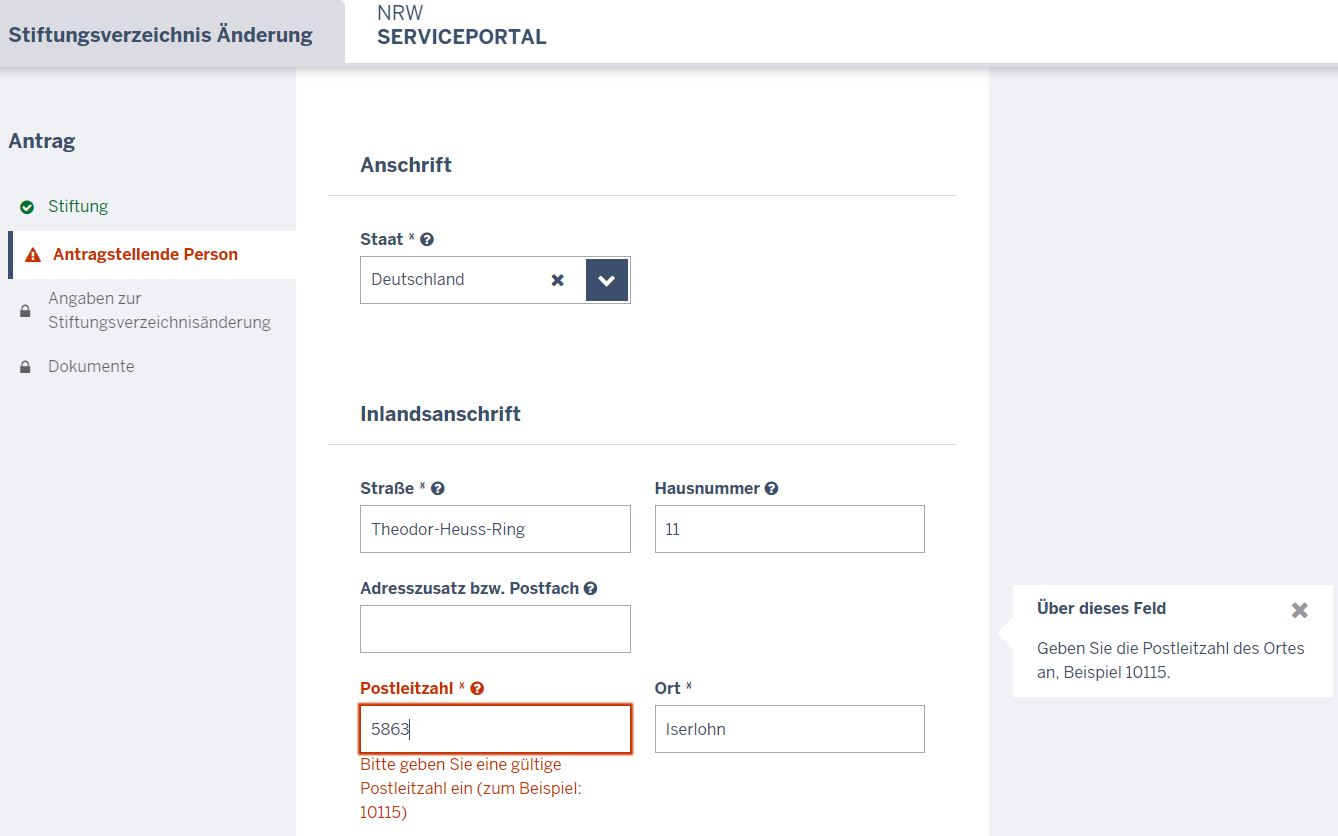
\includegraphics[width=\linewidth]{images/form_adresse.JPG}
  \caption{Ein digitales Formular ``Antrag auf Stiftungsverzeichnis Änderung'', das von der Telekom MMS GmbH modelliert und ins NRW-Serviceportal integriert wurde}
  \label{fig:meineabbildung}
\end{figure}

Um die konkrete Gestaltung und Funktionsweise digitaler Formulare zu veranschaulichen, betrachten wir ein Beispiel (Abb. 2.1). Der Screenshot eines Formularabschnitts aus NRW Serviceportal zeigt typische Merkmale eines digitalen Formulars: eine Navigationsleiste, klar strukturierte und definierte Eingabefelder. Im Gegensatz zu einem Papierformular bietet die digitale Version interaktive Elemente, Dropdown-Menüs für die Auswahl einer Eingabe, Vorbefüllungen persönlicher Daten und Validierungsfunktionen. Hilfetexte und Tooltips sind bereitgestellt, die beim Bedarf den NutzerInnen bei der korrekten Ausfüllung assistieren. Diese Elemente erhöhen nicht nur die Benutzerfreundlichkeit, sondern tragen auch zur Korrektheit und Vollständigkeit der erfassten Daten bei. Der Screenshot stellt somit dar, wie Formulare im eGovernment-Bereich gestaltet sind, um eine effiziente, fehlerfreie und benutzerorientierte Datenerfassung zu ermöglichen. \\

Die Entwicklung und Verwaltung solcher komplexen digitalen Formulare erfordert ein leistungsfähiges Formularmanagementsystem (FMS). Im nächsten Abschnitt wird detailliert erklärt, was ein FMS ausmacht, welche Komponenten zur Verfügung stehen und wie es zur Effizienzsteigerung und Kundenorientierung in der digitalen Verwaltung beiträgt.







% Im Jahre 1450 hat die Geschichte von Formularen mit einem Ablassbrief begonnen. Im Laufe der Zeit hat das Papierformular sein Gestalt immer wieder verändert, von Ablassbrief (1455) über Steuerformulare (1792) und Passagierlisten (1892) bis hin Verwaltungsformulare (1929). Einen digitalen Datenverarbeitungswandel ab der 70er Jahren bezeugte  EDV-Formulare, die viele Vorteile mit sich brachten. Und heute haben wir zwei Begriffe, die die Formularen einen ganz neuen Glanz verleihen : eCommerce und eGovernment. \citep{formulare_schwesinger_2007}\\

% \textbf{Definition: }\textit{``Formulare sind von einer Ordnung bereitgestellte und im Rahmen dieser Ordnung verwaltete Texte mit Lücken, die von individuellen Fällen ausgefüllt werden, die von dieser Ordnung gesucht werden oder diese Ordnung in Anspruch nehmen.'' \cite[S. ~3]{plener_formular_2021}}   \\

% In dieser Arbeit wird über Formulare des eGorvernments gesprochen. Wie in \cite[S.~VI]{plener_formular_2021} gesagt wurde: ``Das Medium \textit{"`Formular"'} transformiert also nicht nur Daten, sondern eine Gestalt von Bürokratie und bürgerlicher Partizipation.'', daher werden auch die Verwaltungdienste in Deutschland kundenorientierter gestaltet und digitalisiert. \\


% Formulare sind Dokumente oder digitale Schnittstellen, die von Bürgern und Unternehmen genutzt werden, um Informationen an die Einrichtungen zu übermitteln. Sie dienen dazu, verschieden Anliegen, Anträge, Meldungen und Informationen zu erfassen und zu verarbeiten. \\
\section{Formularmanagementsystem form.io}

FMS ist eine zentrale und redundanzfreie Formularverwaltung. Es bietet eine einfachere Erstellung von digitalen Formularen an, erfüllt die Anforderungen der barrierefreien Informationstechnik-Verordnung des Bundes, spart Zeit, Papier und Geld. Es ist ein Werkzeug, das für Organisationen und Institutionen konzepiert wurde, die eine Vielzahl von Online-Formularen modellieren und verwalten müssen. Dies umfasst solcher Anwendern wie Unternehmen, Gesundheitswesen, Bildungseinrichtungen, Finanzinstitute, öffentliche Verwaltung und Regierungsbehörden. \\

Die Telekom MMS GmbH verwendet als Grundlage für die Digitalisierung der Verwaltungsdienste eine leistungsstarke FMS einer Firma Form.io \citep{formio}. Durch ihre Flexibilität und umfangreiche Anpassungsmöglichkeiten werden die Anforderungen des OZG erfüllt.\\


\textcolor{red}{Form.io ist eine Plattform für Formularerstellung und Datenmanagement und bietet eine Schlüssel-Komponenten- sowie Nutzer- und Datenverwaltungsinfrastruktur an}. Sie ermöglicht, Formulare mit einem Drag-and-Drop-Baukasten (Komponenten) zu erstellen. Der Baukasten ist einzigartig, weil mit ihm nicht nur HTML-Formulare erstellt, sondern auch JSON-Schemata-Darstellungen der Formularen für die Anwendungsentwicklung erzeugt werden können.\\
% hier noch mal die Nutzer und Datenverwaltung angehen.

\textcolor{red}{Einer der wichtigsten Unterschiede zwischen Form.io und anderen Formularprodukten dabei ist die Art und Weise, wie die Formulare in der Anwendung gerendert werden. Die meisten Plattformen rendern Formulare auf  dem Server (unter Verwendung von Technologien wie PHP, .NET, Java usw.) und senden dann den gerenderten Formular-HTML-Code an Browser.} Dieser Ansatz hat viele Probleme beim Round-Trip-Zeiten, Skalierbarkeit und Flexibilität. Um die neuen Progressive Web Application (PWA), die heute entwickelt werden, bedienen zu können, hat Form.io die Art völlig neu definiert, damit sie flexibel, erweiterbar und performant sind. Formulare, die mit dem Form.io Builder erstellt werden, werden als JSON-Schemata dargestellt, die dann direkt in der Anwendung mithilfe einer JavaScript-Rendering-Engine gerendert werden.\\


Neben der Plattform stellt Form.io eigene Bibliotheken und Integrationen bereit, die in verschiedene Frameworks wie Angular, Vue, React unterstützt werden. Hier sind einige davon:
\begin{itemize}
    \item \textbf{Command Line Interface (CLI):} Für die Interaktion mit Form.io über die Kommandozeile.
    \item \textbf{Webhook Receiver:} Für die automatisierte Nachrichten oder Daten von einem Webhook zu empfangen. Ein Webhook ist eine Methode, mit der eine Anwendung oder ein Dienst Echtzeit-Informationen an andere Anwendungen oder Dienste übermitteln kann, sobald ein bestimmtes Ereignis eintritt.
    \item \textbf{File Upload Proxy Server:} Diese Bibliothek bietet einen Upload-Server/Proxy für die Verwendung mit der Form.io Dateikomponente und URL-Konfiguration. Dies ermöglicht das Hochladen und Herunterladen privater Dateien durch Senden, basierend auf seinem Zugriff auf das Senden des Formulars bzw. das Abrufen des Übermittlungs-JSON. 
    \item \textbf{JavaScript API:} Eine Schnittstelle, um mit den Form.io APIs innerhalb einer JavaScript-Anwendung zu kommunizieren. Beispiel:
    \begin{adjustwidth}{-5em}{0pt}
    \begin{lstlisting}[language=HTML]
        <script src="https://cdn.form.io/formiojs/formio.min.js"></script>
        <script type="text/javascript">
            // Load a form.
            const formio = new Formio('https://formio.com/myproject');
            formio.loadForms().then((forms) => {
              console.log(forms);
            });
        </script>
    \end{lstlisting}
    \end{adjustwidth}
    \item \textbf{Form Renderer:} Kernbibliothek zur Darstellung von Form.io Formularen, die aus einem JSON-Schema erstellt wurden. Beispiel:
    \begin{adjustwidth}{-5em}{0pt}
    \begin{lstlisting}[language=HTML]
        <div id="formio"></div>
        <script type="text/javascript">
            Formio.createForm(document.getElementById('formio'), {
                components: [
                {
                    type: 'textfield',
                    key: 'firstName',
                    label: 'First Name'
                },
                {
                    type: 'email',
                    key: 'email',
                    label: 'Email'
                },
                {
                    type: 'button',
                    key: 'submit',
                    label: 'Submit'
                }]
            });
        </script>
    \end{lstlisting}
    \end{adjustwidth}
    \item \textbf{Form Builder:} Ein Werkzeug, das in der Anwendung eingebettet werden kann, um einen Formularbaukasten zur Verfügung zu stellen. Mit diesem können NutzerInnen Formulare direkt in der Anwendung erstellen.
    \begin{adjustwidth}{-5em}{0pt}
    \begin{lstlisting}[language=HTML]
        <div id="builder"></div>
        <script type="text/javascript">
            Formio.createForm(document.getElementById('builder'), {}, {});
        </script>
    \end{lstlisting}
    \end{adjustwidth}
    \item \textbf{Form Embedding:} Ermöglich die Einbettung eines Formulars in der Anwendung durch Einbindung eines einzigen Script-Tags
    \begin{adjustwidth}{-5em}{0pt}
    \begin{lstlisting}[language=HTML]
        <script src="https://cdn.form.io/formiojs/formio.embed.min.js?src=https://examples.form.io/examples"></script>
    \end{lstlisting}
    \end{adjustwidth}
    Dies ermöglicht es, Formulare von Form.io direkt und ohne großen Entwicklungsaufwand in die Webseite zu integrieren.
    \item \textbf{Form Utilities:} Eine Sammlung von nützlichen JavaScript-Hilfsmitteln, die häufig benötigten Funktionen in Anwendungen anbietet. Sie ist ein Teil des formiojs Bibliothek. Beispiel:
    \begin{adjustwidth}{-5em}{0pt}
    \begin{lstlisting}[language=HTML]
        <script type="text/javascript">
            var utils = require('formiojs/utils');
            utils.eachComponent(form.components, component => {
                // Do something...
            })
        </script>
    \end{lstlisting}
    \end{adjustwidth}
\end{itemize}

Nachdem das umfassende Ökosystem von Form.io und seine Möglichkeiten erläutert wurden, ist es wesentlich, die vielseitigen Komponenten von Form.io zu betrachten. Ein weiterer Aspekt von Form.io ist die Möglichkeit, jede Komponente individuell zu gestalten. Von einfachen Textfeldern und Auswahloptionen bis hin zu komplexeren Elementen wie Datumsauswahlen und Dateiuploads - jede Komponente kann modifiziert und in das Formular integriert werden.

... beschreiben, welche Komponenten es gibt.

... beschreiben, welcher Komponente wird als Grundlage für die Integration genommen wird.

... Übergang zur Geodaten









% Form.io ist ein webbasiertes Tool, das für die schnelle Erstellung und effiziente Verwaltung von Online-Formularen entwickelt wurde. Es kombiniert Formularmodellierung und Datenmanagement in einer einzigen Anwendung, welche eine Integration in diverse Softwareumgebungen ermöglicht.

% Dieses Schema wird dann verwendet, um das Formular dynamisch in Serverlose-Anwendungen (wie Angular, React usw.) zu rendern und gleichzeitig eine REST-API zur Unterstützung dieses Formulars automatisch zu generieren
\section{Geodaten}

Geodaten sind in heutigen Zeit allgegenwärtig und spielen eine zentrale Rolle in der Wirtschaft, Wissenschaft, öffentlicher Verwaltung sowie im privaten Leben. Diese Daten sind digitale Darstellung räumlicher Informationen, die einen direkten und indirekten Raumbezug zur Erdoberfläche haben. Diese Daten beschreiben Lage und Beziehungen zwischen verschiedenen Geoobjekten sowie qualitative und quantativen Merkmale dieser Objekte.\\

Geoobjekte sind räumliche Elemente, die zusätzlich zu Sachinformationen geometrische und topologische Eigenschaften besitzen und zeitlichen Veränderungen unterliegen können. Es handelt sich dabei um physische Objekte wie Gebäude, Straßen, Flüsse, Berge, Städte oder auch um abstrakte Elemente wie Verwaltungsgrenzen, Postleitzahlgebiete etc. Geoobjekte werden auf der Erdoberfläche im Form von Punkten, Linien und Polygonen dargestellt \citep{de_lange_geoinformatik_2020}.

\begin{itemize}
    \item Die \textbf{geometrische Eigenschafen} sind die Informationen zur absoluten Lage und zur Form des Objektes auf der Erdoberfläche.
    \item Die \textbf{topologischen Eigenschaften} beschreiben Umgebung bzw. Umgebungsbeziehungen, Nachbarschaften bzw. Nachbarschaftsbeziehungen, Teilmengen oder Überlagerungen. Die Geoobjekte können verschiedene Sachthemen aufweisen und zudem eine zeitliche Variabilität besitzen.
\end{itemize}

Für die Erhebung von Geodaten ist ein \textbf{Raumbezug} notwendig. D.h., dass Geoobjekten eine bestimmte Position auf der Erde und ein Verhältnis zu anderen Geoobjekten zugeordnet werden kann. Dafür wurden Modelle entwickelt, die sich der Figur der Erde möglichst genau annähern und mathematisch erfassbar sind. \\

Geodaten werden durch ihren Standort auf der Erde beschrieben. Es gibt viele Quellen für Geodaten (z. B. Fernerkundung, Punktwolkendaten, LiDAR, GPS, Internet, IoT usw.), die mit unterschiedlichen Auflösungen und Eigenschaften erfasst werden. Zwei große Kategorien sind Rasterdaten und Vektordaten. Die geografischen Merkmale auf der Erdoberfläche können in Form von Punkten, Linien und Polygonen dargestellt werden, und ihre Koordinaten werden durch Geoinformationssystem (Abschnitt. 2.5) verarbeitet und dargestellt.\\

\textbf{Vektordatenmodell} beschreibt raumbezogene Objekte anhand von Punkten, die in Form von Koordinaten definiert werden. Die Punkte werden genutzt, um Objektgeometrie zu erfassen. Ein Vektor ist nach lateinischer Übersetzung ein „Träger“ oder auch „Fahrer“ von geometrischen Informationen. \textbf{Rasterdatenmodell} stellt raumbezogene computerlesbare Geodaten mit bildhaftem Informationsgehalt dar. Die Geoinformationen werden in Pixel zerlegt. Durch die Verknüpfung von Geodaten und Sachdaten entstehen Geoinformationen, d. h. interpretierte Daten mit Raumbezug, die sich auf Orte oder Bereiche der Erdoberfläche beziehen \citep{klaus_geomatik_2023}. Abbildung 2.2 zeigt die schematische Struktur von Geodaten und unterschiedlichen Typen von Geometrie (Punkt, Linien und Polygone). Hier wird ersichtlich, wie Geodaten organisiert werden, um sowohl ihre räumliche Darstellung als auch ihre sachliche Informationen zu erfassen.\\

\begin{figure}[ht]
  \centering
  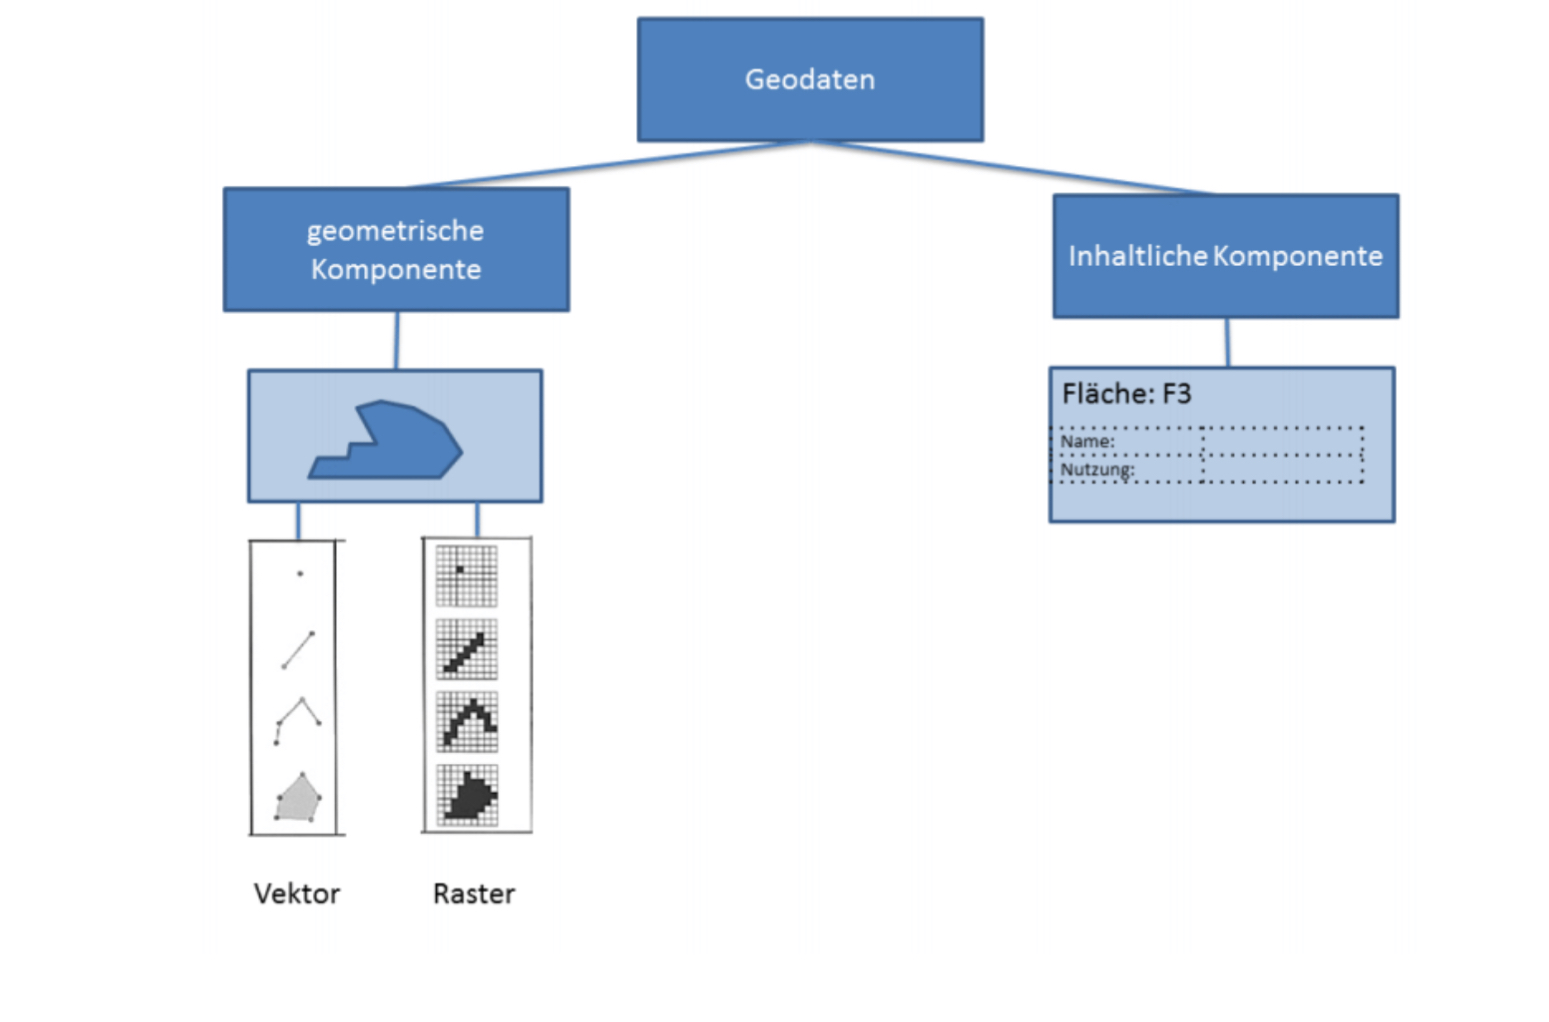
\includegraphics[width=\linewidth]{images/geodaten.jpeg}
  \caption{schematische Darstellung von Geodaten \citep{masterarbeit_fischer}}
  \label{fig:meineabbildung}
\end{figure}

...Weitere Quellen der spezifischen Geodaten\\

In diesem Projekt wird auf die Schulen in Münster, Nordrhein-Westfalen konzentriert. Die erforderlichen Geodaten für diese Schulen und ihre Umgebung sind auf der Webseite von \cite{schulen_geodaten} frei zugänglich und können uneingeschränkt genutzt werden. Die Geodaten sind Schulstandorte in NRW als Shape zum Download gestellt. Für die Speicherung der digitalen Geodaten wurden spezielle Datenbanklösungen entwickelt. Sie werden im nächsten Abschnitt vorgestellt.





% Ein \textbf{geodätisches Koordinatensystem} basiert auf einem mathematischen Model der Erde (Geoid oder Referenzellipsoid) und ermöglicht es, genaue Position (Längen- und Breitengrade) von Geoobjekten zu bestimmen. Es handelt sich dabei um ein globales Referenzsystem, das die Krümmung der Erde berücksichtigt, um präzise Lageinformationen zu liefern.

% \begin{figure}[ht]
%   \centering
%   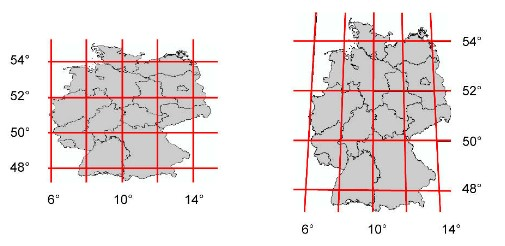
\includegraphics[width=\linewidth]{images/karte-in-deutschland.jpg}
%   \caption{Umrisse der Bundesrepublik Deutschland in einem kartesischen Koordinatensystem und in der winkeltreuen Lambert-Projektion}
%   \label{fig:meineabbildung}
% \end{figure}

% Eine \textbf{Projektion} ist eine Methode, um die dreidimensionale Oberfläche der Erde auf eine zweidimensionale Karte zu übertragen. Da es unmöglich ist, die gekrümmte Oberfläche der Erde ohne Verzerrungen auf eine flache Karte zu projizieren, gibt es verschiedene Projektionsarten, die je nach Anwendung und Region unterschiedliche Eigenschaften und Verzerrungen aufweisen.

% \begin{figure}[ht]
%   \centering
%   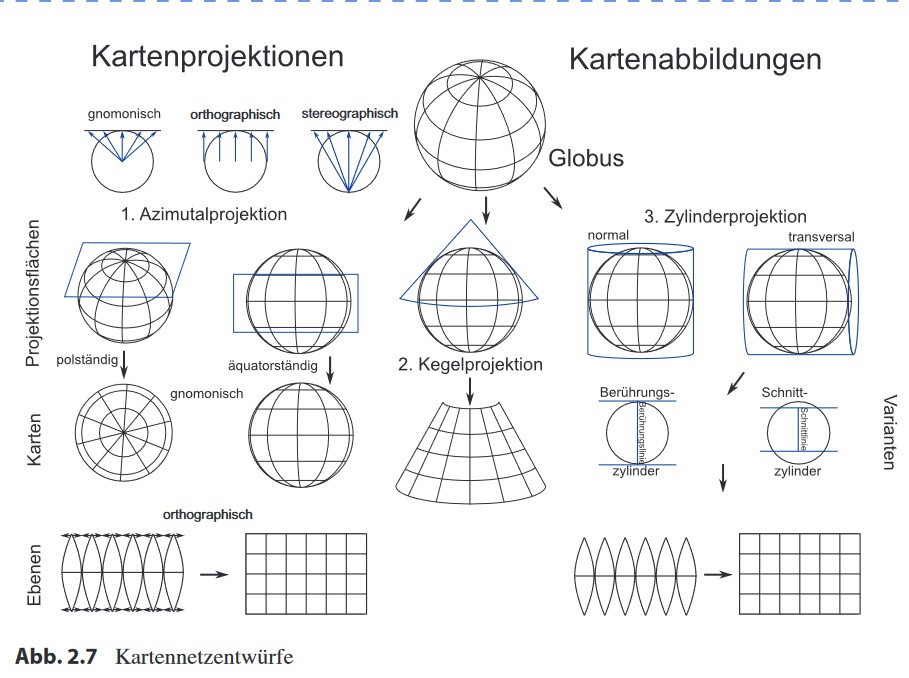
\includegraphics[width=\linewidth]{images/Kartennetzentwurfe.jpg}
%   \caption{Kartennetzentwürfe}
%   \label{fig:meineabbildung}
% \end{figure}

% Das geodätische Lagekoordinationssystem bezieht sich auf das System zur Bestimmung der genauen Position von Objekten auf der Erdoberfläche, während eine Projektion die Methode ist, wie diese Position auf eine Karte dargestellt wird.\\



% Geodaten unterscheiden sich in Geobasis- und Geofachdaten.
% Geobasisdaten sind von den amtlichen Vermessungseinrichtungen in einem einheitlichen geodätischen Bezugssystem bereitgestellten topographischen Daten, die die wesentlichen Objekte der Erdoberfläche (Siedlungen, Verkehrsnetze, Vegetation, Gewässer, Geländeformen und Grenzen politischer und administrativer Einheiten) anwendungsneutral beschreiben. Alle erfassten Geobasisdaten werden in digitaler Form im Topographisch-Kartographischen Informationssystem bei den Vermessungsverwaltungen der Länder vorgehalten. (adv-online.de geodatenzentrum.de). Geobasisdaten bilden topographische „Grundgerüst“.

% Geofachdaten sind raumbezogene thematische Daten, die fachgebietsbezogen erfasst und bereitgestellt werden und sich auf alle Gegenstände und Sachverhalte mit geographischem Bezug erstrecken können. Beispiele seien Wetter- und Klimadaten, Daten zum Umweltzustand, Landnutzungsdaten und statische Daten.

% Kartennetzentwürfe sind zweidimensionale Kartendarstellungen der gekrümmten Erdoberfläche.\\

% \begin{figure}[ht]
%   \centering
%   
\includegraphics[width=\linewidth]{images/kartennetz.jpg}
%   \caption{Klassifikation der Kartennetzentwürfe nach der Art der Abbildungsflächen}
%   \label{fig:meineabbildung}
% \end{figure}
\section{Geo-Datenbanken}

Die Speicherung, Verwaltung und Verarbeitung von Daten haben für viele Anwendungsbereiche eine große Bedeutung.  Wie \cite{brinkhoff_geodatenbanksysteme_2022} in seinem Werk über Geodatenbanksysteme erwähnt, erfüllen diese speziellen Datenbanken eine Vielzahl an Aufgaben. Sie müssen nicht nur allgemeine Anforderungen wie Sicherheit, Mehrbenutzerfähigkeit und Effizienz erfüllen, sondern auch spezifische geoinformationssystemische Funktionen bieten. Dazu gehören die Verwaltung von Geometriedaten und deren Verarbeitung. Zudem stellen sie Werkzeuge für die räumlichen Analyse von Geoobjekten bereit und halten sich an Standards, um eine möglichst große Interoperabiltät zu gewährleisten. \\

\textbf{Definition: }Eine Geodatenbank ist eine Datenbank, welche für die Verarbeitung von räumlichen Daten optimiert ist. [...] Geodatenbanken entstehen oft durch die Erweiterung klassischer Datenbanksysteme mit entsprechender Software. Bekannte Ausführungen sind MongoDB with GeoJSON, PostgreSQL with PostGIS, SpatiaLite with Sqlite, Oracle Spatial and Graph etc. \citep{wiki-geodatenbank}.\\

In der Abbildungen 2.2 und 2.3 (eigene Darstellung) wird ein Unterschied der Speicherung von Geodaten gezeigt. Die beide Abbildungen zeigen Tabellen aus einer Geodatenbank, wobei der Hauptunterschied in der Art und Weise liegt, wie die geographischen Koordinaten gespeichert sind. In der ersten Bild werden Koordinaten als separate Spalten für den Längengrad und den Breitengrad aufgeführt. Jede Zeile enthält nummerische Werte für diese Koordinaten, die die genaue Position auf der Erde repräsentiert. Im zweiten Bild wird stattdessen eine Spalte koordinaten mit einem speziellen Geometriedatentyp hinterlegt. Hier sind die Koordinaten als 'POINT' gespeichert. Für jeden Eintrag wird ein Punkt mit dem jeweiligen Längen- und Breitengraden in Klammern angegeben 'POINT(13.357818 52.49637)'. \\

\begin{figure}[ht]
  \centering
  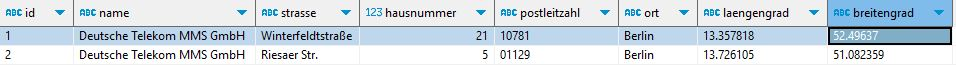
\includegraphics[width=\linewidth]{images/einfacheDB.jpg}
  \caption{Geodaten in der Datenbank. How (not) to}
  \label{fig:meineabbildung}
\end{figure}
\begin{figure}[ht]
  \centering
  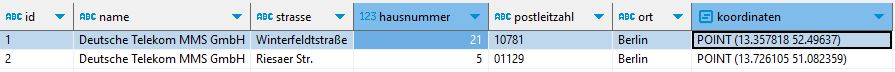
\includegraphics[width=\linewidth]{images/geoDB.jpg}
  \caption{Geodaten in der Datenbank mit Geo-Erweiterug. How to}
  \label{fig:meineabbildung}
\end{figure}
 Die Geodatenbank haben drei Aspekte, die räumliche Daten mit einer Datenbank zu verknüpfen: Datentypen, Indizes und Funktionen.
\begin{enumerate}
    \item Räumliche Datentypen beziehen sich auf solche Formen wie Punkt, Linie, Polygon, Multipolygon.
    \item Die mehrdimensionale räumliche Indizierung ist eine Funktion, die es ermöglicht, räumliche Daten effizient zu organisieren und zu durchsuchen. Diese Indizes sind speziell für die Verarbeitung von Geodaten konzipiert und optimieren Abfragen, die sich auf die Positionen, den Abstand oder Überlappung von Geoobjekten beziehen. Sie beschleunigen die Suchanfragen, indem sie nur die relevanten Teile der Datenbank durchsuchen, anstatt jeden Datensatz einzeln zu prüfen.
    \item Räumliche Funktionen umfassen eine Sammlung von Operationen und Abfragen, die in SQL bereitgestellt sind. Dies Funktionen können verwendet werden, um räumliche Beziehungen zu bestimmen, wie z.B. zu prüfen, ob ein Punkt in einem Polygon liegt, Lienen sich kreuzen oder die nächstgelegenen Objekte zu einem gegebenen Punkt zu finden. Sie ermöglichen es, komplexe räumliche Fragen direkt in der Datenbank zu beantworten. 
\end{enumerate}

Geodatenbanken ermöglichen durch die klassischen SQL-Befehlen Beziehungen zwischen Geometrie zu analysieren bzw. neue Geometrien zu erstellen wie beispielsweise Berechnungen von Längen, Distanzen, Prüfungen auf Bedingungen wie maximaler Abstand, Erstellung neuer Geometrien etc.

\section{Geoinformationssysteme}
\label{sec:GIS}
% Nach \cite{de_lange_geoinformatik_2020} ist ein Geoinformationssystem (GIS) ein Informationssystem, das sich auf Modellierung und digitale Abbildungen von Geoobjekte der realen Welt konzentriert. Dieses System erfasst, verarbeitet, speichert, visualisieret und wertet raumbezogene Informationen aus. Dies erfordert spezielle Werkzeuge und Funktionen. \\

``Ein Geoinformationssystem ist ein rechnergestütztes System, das aus Hardware, Software, Daten und den Anwendungen besteht. Mit ihm können raumbezogene Daten digital erfasst, gespeichert, verwaltet, aktualisiert, analysiert und modelliert sowie alphanumerisch und graphisch präsentiert werden.'' \citep[S. ~375]{de_lange_geoinformatik_2020} GIS konzentriert sich auf Modellierung und digitale Abbildungen von Geoobjekten der realen Welt. Es besteht aus Hardware, Software, Daten und Anwendern. zur Visualisierung von Geodaten werden solche Dienste wie GoogleMaps, OpenStreetMap oder Basemap.de angesporchen. \\


Die Abbildung 2.5 illustriert das Konzept, wie Daten in einem GIS durch die Darstellung verschiedener Schichten organisiert werden, um realen Welt zu digitalisieren. Sie bildet ab, wie die physische Welt in GIS-Datenbank strukturiert wird, um eine Vielzahl von Analysen und Funktionen zu unterstützen. 
\begin{figure}[ht]
  \centering
  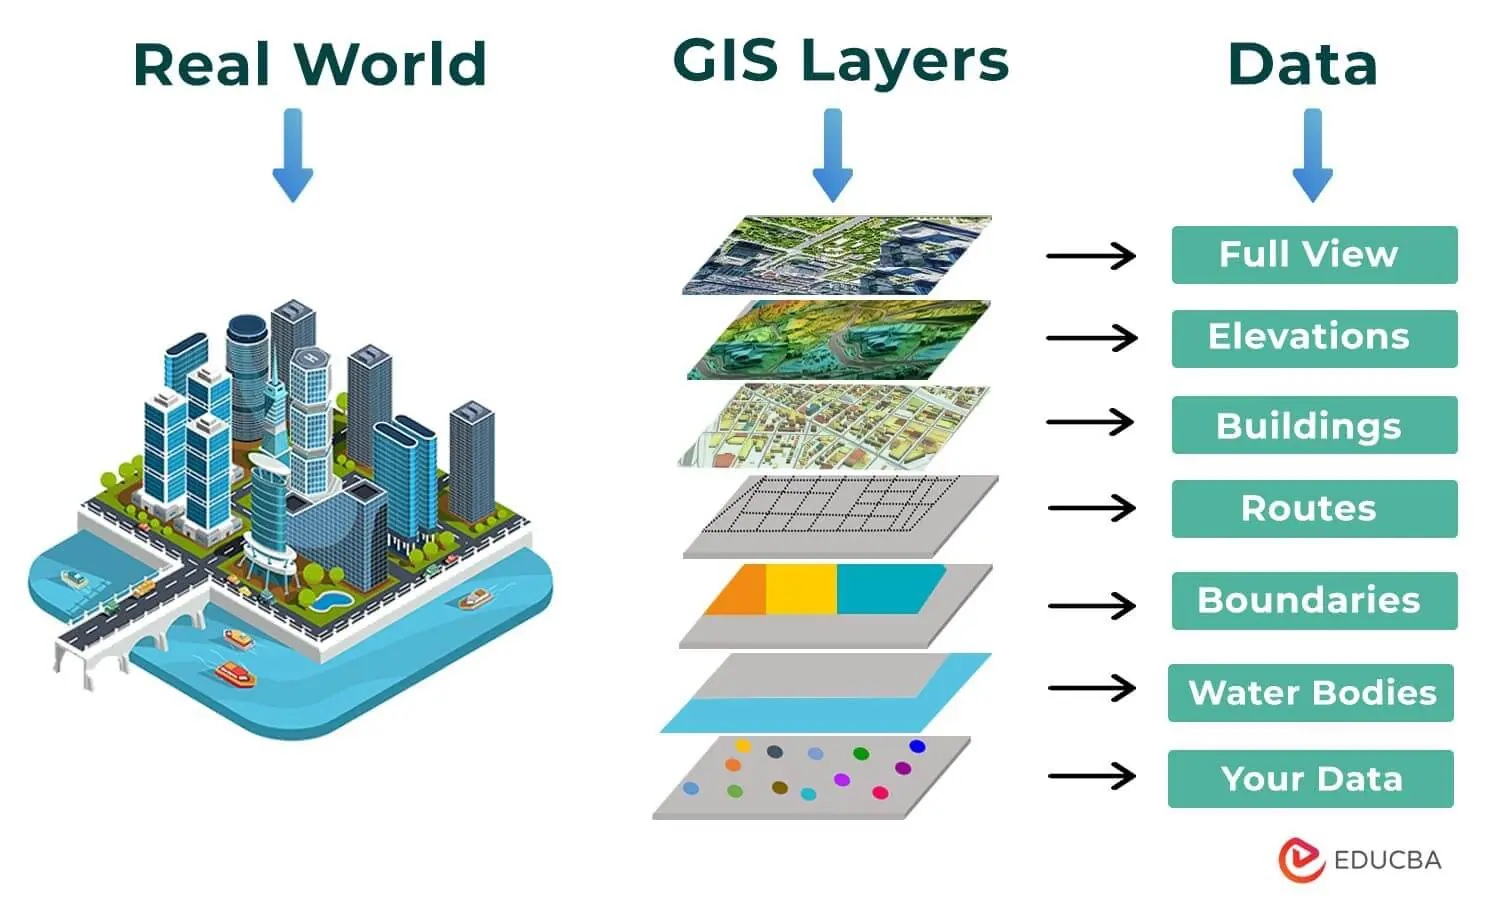
\includegraphics[width=\linewidth]{images/gis.jpg}
  \caption{Konzept der Datenorganisation in einem GIS \citep{gis_bild}}
  \label{fig:meineabbildung}
\end{figure}

Moderne GIS sind vielseitig und bieten eine breite Palette von Funktionen. Hier sind neben Visualisierung weitere Funktionsmöglichkeiten von GIS:
\begin{itemize}
    \item Datenerfassung und -bearbeitung.
    \item Ermittlung von Standorten, Mustern und Beziehungen zwischen verschiedenen Geoobjekten.
    \item Analysieren von Distanzen, Flächen und räumlichen Überlappungen
    \item Sammeln, speichern und verwalten großer Mengen Geodaten.
    \item Integration und Verwaltung verschiedener Datenformate und -quellen.
    \item Erstellung von Routen.
    \item Überwachung und Analyse von Umweltveränderungen und -auswirkungen.
\end{itemize}

In gewerblichen Bereichen dominieren kommerzielle Geoinformationssystem wie ArcGIS und Map3D. Die bekanntesten Open-Source-GIS sind QGIS und GRASS GIS. Es gibt zahlreiche GIS-Werkzeuge wie Openlayers, Leaflet. Online-GIS sind beispielsweise Google Maps, OpenStreetMap. Und die webbasierte GIS sind Server-Software, die auf Geodaten spezialisierte Geodienste zur Verfügung gestellt wie MapServer, Geoserver.\\

Im Rahmen dieser Bachelorarbeit werde ich für das Showcase einen GIS-Modul nach die Anforderungen (Kapitel 3) der Telekom MMS GmbH konzepieren und entwickeln, um eine Karte inklusive Daten von Schulen in einem Schulanmeldung Formular zu visualisieren. Für die Implementierung von GIS wird eine leistungsstarke JavaScript-basierte Bibliothek Openlayers als Werkzeug genutzt. Die wird in nächsten Abschnitt näher erklärt.



\section{Openlayers}


\chapter{Anforderungen}
\label{cha:anforderungen}

Use Case
Die Anmeldung von Kindern an einer Schule erfolgt in Deutschland durch seine Eltern oder andere Erziehungsberechtigte. Dabei gelten bezüglich der Möglichkeiten zur Schulwahl je nach Bundesland Einschränkungen. Insbesondere in Hamburg und NRW gibt es aber eine Möglichkeit zur weitgehend freien Schulwahl: Eltern können sich frei zwischen allen Schulen im Stadt- bzw. Einzugsgebiet entscheiden \citep{schulwahl_nrw}. Ein Kriterium für die Schulwahl kann die Länge bzw. Beschaffenheit des zukünftigen Schulwegs eines Kindes sein. Grundsätzlich ist es aus Bürgersicht wünschenswert, die Schulanmeldung digital vozunehmen anstelle eines Vor-Ort-Termins in der jeweiligen Schule. In diesem Zusammenhang erscheint es sinnvoll, ein Formular zu gestalten, das Karteninformationen enthält, sodass die Eltern sich den zukünftigen Schulweg ihres Kindes anzeigen lassen können.

\section{funktionale Anforderungen}
Nutzer Bürger X
Ziel des Bürgers: Der Bürger will sein Kind an einer Schule anmelden

X möchte eine im Internet zu findende Webseite ansteuern, die ihm ein Formular bereitstellt zur Anmeldung seines Kindes an einer Schule	Muss	Webseite Bürger
X möchte durch klicken eines Buttons auf der Webseite deas Anmeldeformular aufrufen	Muss	Webseite Bürger
X möchte seine Kontaktdaten ins Formular eingeben	Muss	Formular
X möchte den Namen seines Kindes in das Formular eingeben	Muss	Formular
X möchte die Wohnadresse seines Kindes im Formular angeben	Muss	Formular
X möchte die Wohnadresse des Kindes auf einer Karte dargestellt sehen (z.B. durch einen Pfeil markiert)	Muss	GIS 
X möchte alle Schulen in einem Umkreis A um seine Wohnadresse angezeigt bekommen	Muss	GIS
X möchte anhand eines Eingabefeldes im Formular den Umkreis A zwischen 1 und 50 km ändern können	Soll	Formular
X möchte die angezeigten Schulen nach Schultyp filtern können	Soll	GIS / Formular
X möchte eine Schule auswählen können durch Klicken in die Karte	Muss	GIS
X möchte die Laufdistanz zu der ausgewählten Schule angezeigt bekommen	Soll	GIS
X möchte anhand eines Auswahlfeldes wählen ob er die Distanz via Auto, per Fahrrad oder zu Fuß zurücklegen wird	Soll	GIS
X möchte die Distanz via Auto, Fahrrad oder zu Fuß angezeigt bekommen	Soll	GIS
X möchte auswählen können die Distanz via ÖPNV zurückzulegen	Kann	GIS
X möchte zusätzlich die Fahrzeit via ÖPNV angezeigt bekommen	Kann	GIS
X möchte die von ihm für sein Kind gewünschte Schule benennen können (Schule1)	Muss	Formular
X möchte eine Alternative (Schule2) wählen können, falls sein Kind Schule1 nicht besuchen kann	Kann	Formular
X möchte dan Anmeldeprozess durch Klicken eines Buttons abschließen können	Muss	Formular


Nutzer Sachbearbeiter Y
Ziel des Sachbearbeiters: Er möchte erkennen wieviele Anmeldungen pro Schule vorliegen und zusätzliche Daten wie z.B. Weglängen abfragen

Y möchte eine Karte seines Zuständigkeitsbereichs auf einer Webseite sehen	Muss	Webseite Sachb.
Y möchte alle Schulen (seines Zuständigkeitsbereichs) auf einer Karte sehen	Muss	GIS
Y möchte die Anzahl aller Anmeldungen für jede Schule auf der Karte angezeigt bekommen	Muss	GIS
Y möchte, dass alle Schulen mit mehr Anmeldungen als Plätzen in Rot markiert werden	Soll	GIS
Y möchte eine Schule x auswählen können und die Wohnorte aller Anmeldungen in Farbe x angezeigt bekommen	Soll	GIS
Y möchte eine zweite Schule y auswählen können und die Wohnorte aller Anmeldungen in Farbe y angezeigt bekommen 	Soll	GIS

\section{nicht-funktionale Anforderungen}


% Was sind die Anforderungen?
% funktionale und nicht-funktionale Anforderunge



\chapter{Konzeption}
\section{Architektur}
\section{Inhalte}

\chapter{Implementierung des GIS-Showcases}
% \begin{enumerate}
%     \item Wie kann ich meine Frage beantworten?
%     \item Welche Methode in welchem Zeitraum mit wievielen Menschen / Quellen / ...
%     \item werde ich anwenden?
%     \item Wie setze ich die Anforderungen um?
% \end{enumerate}
\section{Backend}
\section{Datenbank}
\section{Frontend}






\chapter{Evaluation}
% prüfen, ob die Anforderungen erfüllt sind

\section{Auswertung}
% -Was bedeutet meine Implementierung, wenn ich sie mit den Anforderungen vergleiche? 
% Sind die Anforderungen erfüllt?
\section{Zusammenfassung der wichtigen Erkenntnisse}
\section{Handlungsempfehlungen für zukünftige Entwicklung}
\section{Ausblick auf weitere Anwendungsbereiche des GIS-Showcases}

% - Was habe ich geleistet und warum ist das gut?
% - Was habe ich nicht geleistet und warum?
% - Was ist das Wichtigste aus den Ergebnissen meiner Arbeit, das auch andere wissen sollten?
% - Was könnte beim nächsten Mal anders/besser gemacht werden?
% - Welche Fragen haben sich ergeben, was könnte man im Anschluss noch herausfnden oder entwickeln?

\chapter{Fazit}
\section{Zusammenfassung}
\section{Handlugnsempfehlungen}
\section{Ausblick}
% Das Konzept des ``Renderns'' von Formularen, das Form.io verwendet, ist ein zentraler Aspekt moderner Webanwendungen, insbesondere von Progressive Web Applications (PWAs). Hier ist eine detaillierte Erklärung der verschiedenen Aspekte dieser Herangehensweise:

Serverseitiges Rendering: Traditionelle Webanwendungen generieren oft das HTML für ein Formular auf dem Server. Das bedeutet, dass der Server die Logik ausführt, um das komplette HTML zu erstellen, und dieses dann an den Browser des Benutzers sendet. Das kann zu Problemen führen, zum Beispiel mit der Ladegeschwindigkeit, da der Browser auf die Verarbeitung durch den Server warten muss, und mit der Flexibilität, da Änderungen im Formular oftmals einen erneuten Serveraufruf erfordern.

JSON-Schema: Anstatt HTML-Code für ein Formular zu erzeugen, verwendet Form.io ein JSON-Schema. Ein JSON-Schema ist eine strukturierte Datenbeschreibung in einem standardisierten Format. Es definiert die Form und die Daten eines Formulars, einschließlich der Feldtypen, Validierungsregeln und anderer Einstellungen.

JavaScript-Rendering-Engine „Form Renderer“: Das JSON-Schema des Formulars wird durch eine clientseitige JavaScript-Bibliothek, den „Form Renderer“, verarbeitet. Anstatt auf den fertig gestellten HTML-Code vom Server zu warten, nimmt die Rendering-Engine das JSON-Schema und baut daraus dynamisch das Formular im Browser des Benutzers auf.

Vorteile für Progressive Web Applications (PWAs): Dieser Ansatz ist besonders vorteilhaft für PWAs, die darauf ausgelegt sind, schnell und reaktionsschnell zu sein, auch auf mobilen Geräten mit langsamer Internetverbindung. Da das Formular clientseitig gerendert wird, kann es schnell neu gezeichnet werden, wenn sich Daten ändern, ohne dass eine Verbindung zum Server notwendig ist. Das verbessert die Performance und bietet ein nahtloseres Erlebnis für den Benutzer.

Flexibilität und Erweiterbarkeit: Da das Formular aus JSON-Schema erzeugt wird, können Entwickler das Formular leicht anpassen, indem sie das Schema ändern. Sie können neue Felder hinzufügen, Regeln für die Validierung anpassen oder das Layout ändern, ohne den Servercode zu ändern oder das Formular neu vom Server laden zu müssen.

Open Source: Dass Form.io seinen Form Renderer als Open-Source-Bibliothek auf GitHub zur Verfügung stellt, bedeutet, dass Entwickler die Bibliothek frei verwenden, anpassen und verbessern können. Sie profitieren von der Gemeinschaft, die Fehler behebt und neue Funktionen hinzufügt, was zur Robustheit und Sicherheit des Tools beiträgt.

Zusammengefasst bedeutet das clientseitige Rendering von Formularen durch Form.io, dass Entwickler leistungsfähige, interaktive und leicht anpassbare Formulare erstellen können, die für moderne Webanwendungen, insbesondere PWAs, geeignet sind.

Serverseitige Formularverarbeitung ist ein traditioneller Ansatz, bei dem die Logik zur Verarbeitung der Formulardaten auf dem Webserver stattfindet. Hier ist ein einfaches Beispiel für die Verwendung von PHP, einer gängigen Sprache für serverseitige Programmierung:

PHP-Code (serverseitig):
\begin{lstlisting}[language=PHP]
    <?php
        // Ein einfaches serverseitiges Skript, das ein Formular verarbeitet
        // Ueberpruefen, ob das Formular gesendet wurde
        if ($_SERVER["REQUEST_METHOD"] == "POST") {
            // Sammeln der Formulardaten
            $name = $_POST['name'];
            $email = $_POST['email'];
        
            // Einfache Validierung
            if (empty($name)) {
                echo "Name ist erforderlich.";
            } else if (!filter_var($email, FILTER_VALIDATE_EMAIL)) {
                echo "Ungueltige E-Mail-Adresse.";
            } else {
                // Datenverarbeitung
                // Zum Beispiel: Speichern der Daten in einer Datenbank
            }
        }
    ?>
\end{lstlisting}
\begin{lstlisting}[language=HTML]
    <!-- Das HTML-Formular, das an das PHP-Skript gesendet wird -->
    <form action="form_process.php" method="post">
        Name: <input type="text" name="name">
        E-Mail: <input type="text" name="email">
        <input type="submit" value="Submit">
    </form>
\end{lstlisting}

In diesem Beispiel würde das Formular <form> an die PHP-Datei form-process.php gesendet, wenn der Benutzer auf ``Submit'' klickt. Das PHP-Skript würde dann die Daten validieren und entsprechend verarbeiten, beispielsweise in einer Datenbank speichern.

Die Probleme mit diesem Ansatz sind:
\begin{itemize}
    \item Round-Trip-Zeiten: Jedes Mal, wenn das Formular gesendet wird, muss der Browser auf eine Antwort vom Server warten, was zu einer längeren Wartezeit führen kann, insbesondere bei langsamen Netzwerkverbindungen.
    \item Skalierbarkeit: Bei vielen gleichzeitigen Nutzern kann der Server durch das Rendern von Formularen belastet werden.
    \item Flexibilität: Änderungen am Formularlayout oder an der Logik erfordern oft eine Aktualisierung des Server-Codes und ein erneutes Deployment.
\end{itemize}

Im Gegensatz dazu, bei der clientseitigen Verarbeitung mit Form.io, wird das Formular im Browser des Benutzers gerendert und verarbeitet, was viele dieser Probleme mildert.
% 
\paragraph{Webhook Receiver}
Ein Webhook Receiver, auch bekannt als Webhook Endpoint, ist ein Bestandteil in der Programmierung und im Webdesign, der es ermöglicht, automatisierte Nachrichten oder Daten von einem Webhook zu empfangen. Ein Webhook ist eine Methode, mit der eine App oder ein Dienst Echtzeit-Informationen an andere Anwendungen oder Dienste übermitteln kann, sobald ein bestimmtes Ereignis eintritt.
Um zu verstehen, wie ein Webhook Receiver funktioniert, hier ein einfaches Beispiel:
Ereignis: In einer Anwendung tritt ein bestimmtes Ereignis ein, beispielsweise ein neuer Verkauf in einem Online-Shop.
Webhook: Der Online-Shop ist so konfiguriert, dass er bei jedem Verkauf einen Webhook auslöst. Dieser Webhook sendet Daten über den Verkauf (wie Details zum gekauften Artikel, zum Käufer usw.) an eine vordefinierte URL.
Webhook Receiver: An der empfangenden URL befindet sich der Webhook Receiver. Dies ist eine speziell eingerichtete Komponente auf einem Server, die darauf wartet, Daten von Webhooks zu empfangen. Sobald die Daten eintreffen, verarbeitet der Receiver sie entsprechend – beispielsweise indem er sie in einer Datenbank speichert, eine Benachrichtigung sendet oder eine andere Aktion auslöst.

Der Vorteil von Webhooks und ihren Receivern liegt in ihrer Effizienz und Echtzeit-Fähigkeit. Anstatt dass eine Anwendung regelmäßig eine andere Anwendung abfragen muss, um zu sehen, ob es neue Daten oder Updates gibt (was Ressourcen verbraucht und zu Verzögerungen führen kann), sendet der Webhook die Informationen sofort, wenn das Ereignis eintritt. Dies macht Webhooks zu einem wichtigen Werkzeug für die Integration und Automatisierung von Prozessen in modernen Webanwendungen.
Webhook Receiver sind eine effiziente Methode, um Echtzeit-Updates zwischen verschiedenen Systemen oder Anwendungen zu ermöglichen. Es gibt jedoch auch andere Techniken und Methoden, die für ähnliche Zwecke verwendet werden können. Einige Alternativen zu Webhook Receivern sind:

Polling: Bei dieser Methode fragt eine Anwendung in regelmäßigen Abständen eine andere Anwendung oder einen Server ab, um zu überprüfen, ob neue Daten oder Updates vorliegen. Polling ist einfach zu implementieren, kann aber ineffizient sein, da es Ressourcen verbraucht, auch wenn keine neuen Daten verfügbar sind.

Long Polling: Eine Verbesserung des herkömmlichen Pollings. Hierbei hält der Server eine Anfrage offen, bis neue Daten verfügbar sind. Dies reduziert die Anzahl der Anfragen im Vergleich zum normalen Polling, kann aber immer noch weniger effizient als Webhooks sein.

WebSocket: Eine Technologie, die eine dauerhafte Verbindung zwischen Client und Server ermöglicht. Über diese Verbindung können Daten in Echtzeit in beide Richtungen übertragen werden. WebSockets eignen sich besonders gut für Anwendungen, die kontinuierliche Datenströme benötigen, wie beispielsweise Chat-Anwendungen oder Live-Streaming-Dienste.

Server-Sent Events (SSE): Eine Technik, bei der der Server automatisch Daten an den Client sendet, sobald neue Informationen verfügbar sind. SSE wird hauptsächlich für unidirektionale Kommunikation vom Server zum Client verwendet.

Message Queues und Message Brokers: Systeme wie RabbitMQ, Apache Kafka oder AWS SQS ermöglichen es Anwendungen, Nachrichten in einer Warteschlange zu speichern und sie zu verarbeiten, wenn der Empfänger bereit ist. Diese Methode ist besonders nützlich, um Lastspitzen zu bewältigen und die Entkopplung von Diensten zu ermöglichen.

Jede dieser Methoden hat ihre eigenen Vor- und Nachteile und eignet sich für unterschiedliche Anwendungsfälle. Die Wahl der richtigen Methode hängt von den spezifischen Anforderungen der Anwendung ab, wie der Notwendigkeit von Echtzeit-Updates, der Art der Datenübertragung und der Skalierbarkeit.


\appendix
\input{appendix/apA} % Appendix A
\backmatter
\bibliographystyle{apalike}
\bibliography{data/literaturverzeichnis}
\end{document}
